%%%%%%%%%%%%%%%%%%%%%%%%%%%%%%%%%%%%%%%%%%%%%%%%%%%%%%%%%%%%%%%%%%%%%%%%%%%%%%%%
%
%
%
%%%%%%%%%%
\begin{appendices}


%%%%%%%%%%%%%%%%%%%%%%%%%%%%%%%%%%%%%%%%%%%%%%%%%%%%%%%%%%%%%%%%%%%%%%%%%%%%%%%%
%
%
%
%%%%%%%%%%
\chapter{Abbildungen}

% Grundlagen - Geometrie - Gleichseitiges Dreieck

\begin{figure}[h!]
	\centering
	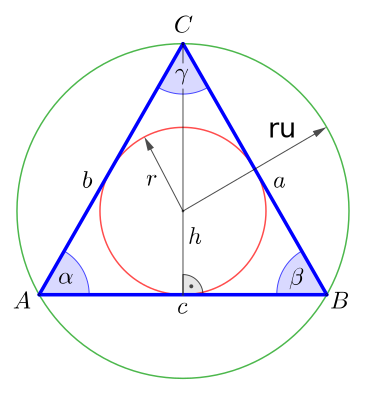
\includegraphics[width=0.45\linewidth]{wikipedia_gleichseitiges_dreieck}
	\captionwithcite{Ein gleichseitiges Dreieck.}{\cite{wikipedia2018dreieck}}
	\label{fig:wikipedia_gleichseitiges_dreieck}
\end{figure}


% Grundlagen - Geometrie - Regelmäßiges Fünfeck

\begin{figure}[h!]
	\centering
	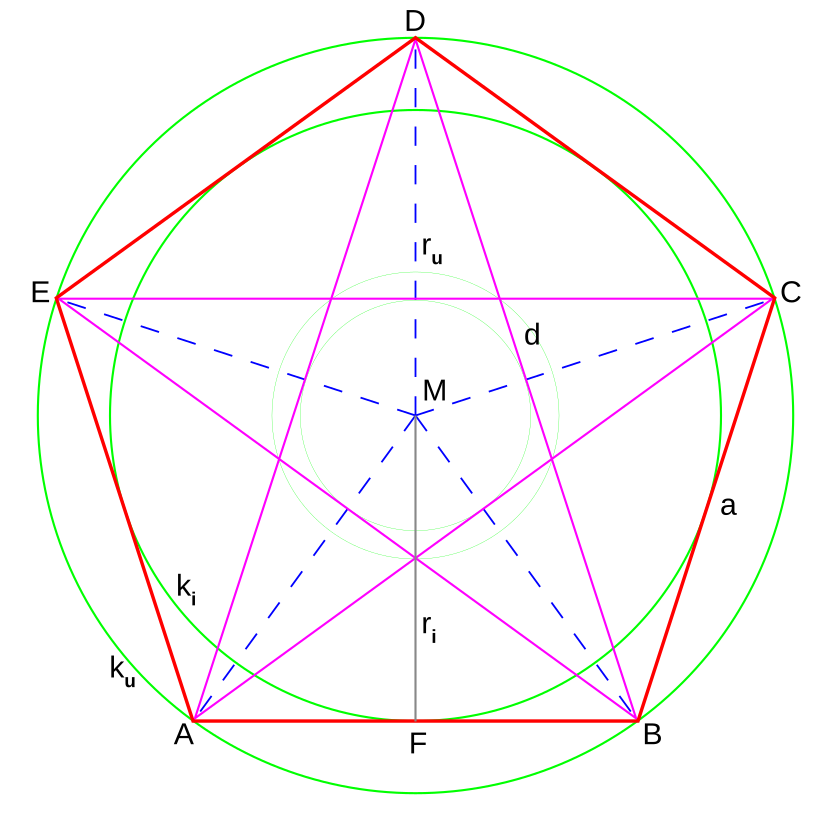
\includegraphics[width=0.45\linewidth]{wikipedia_regelmaessiges_fuenfeck}
	\captionwithcite{Ein regelmäßiges Fünfeck in rot und ein Pentagramm in violett.}{\cite{wikipedia2018fuenfeck}}
	\label{fig:wikipedia_regelmaessiges_fuenfeck}
\end{figure}


% Evaluation - Trajektorie

\begin{figure}[h!]
	\centering
	\begin{subfigure}{0.49\linewidth}
		\centering
		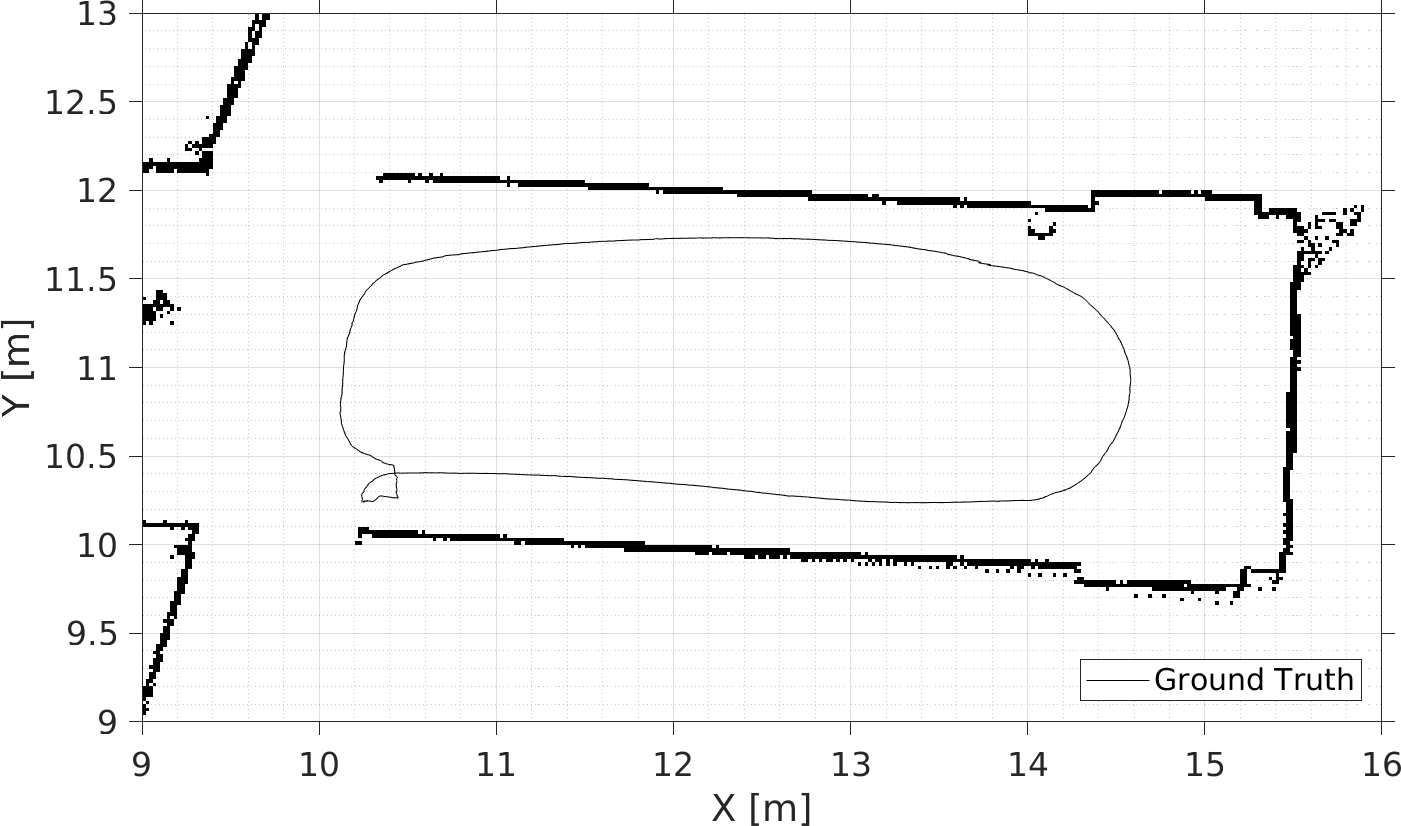
\includegraphics[width=\linewidth]{Record_2018-02-08-12-30-43_trajectory1}
		\caption{Ground Truth}
		\label{fig:Record_2018-02-08-12-30-43_trajectory1}
	\end{subfigure}
	\hfill
	\begin{subfigure}{0.49\linewidth}
		\centering
		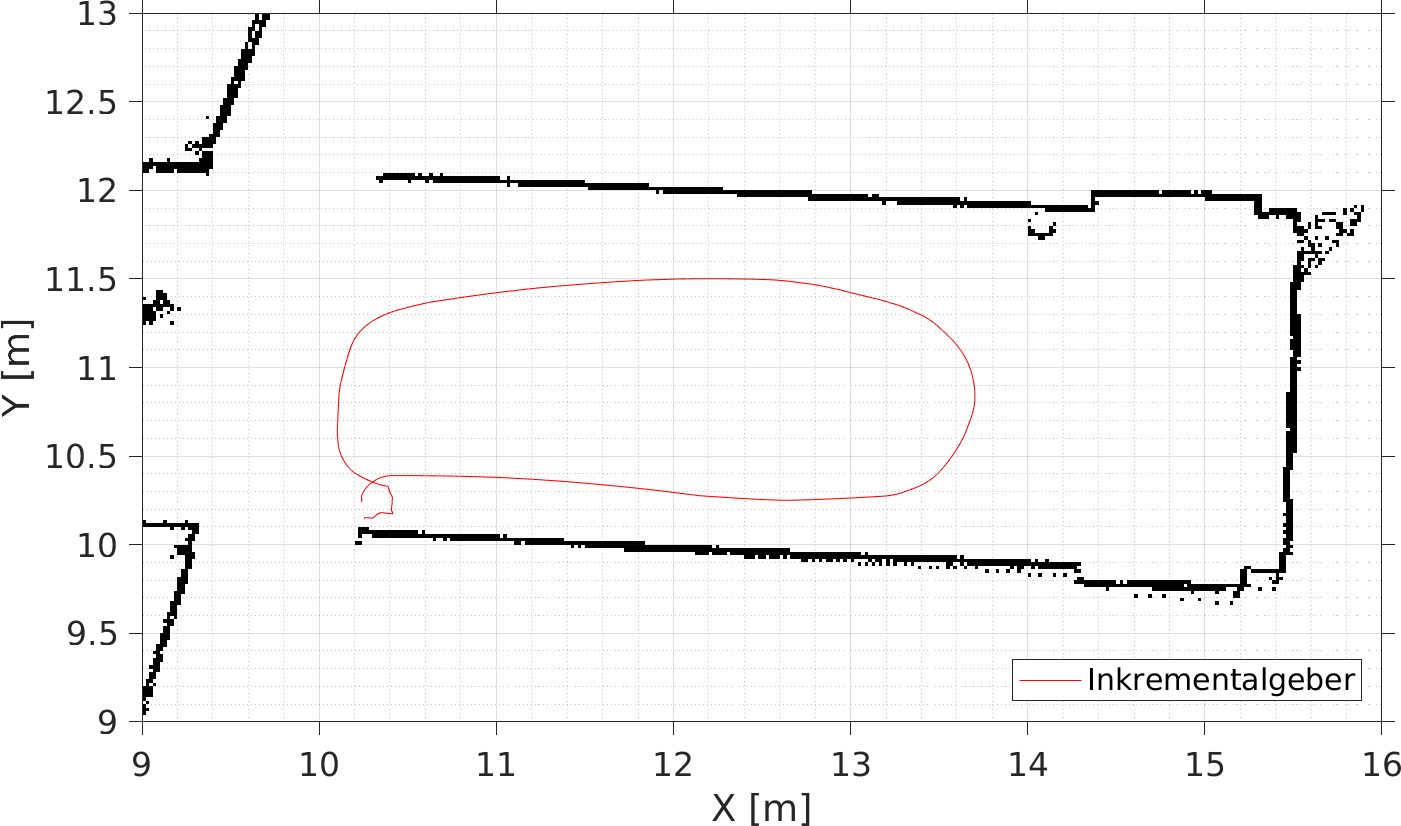
\includegraphics[width=\linewidth]{Record_2018-02-08-12-30-43_trajectory2}
		\caption{Inkrementalgeber}
		\label{fig:Record_2018-02-08-12-30-43_trajectory2}
	\end{subfigure}
	\par
	\bigskip
	\begin{subfigure}{0.49\linewidth}
		\centering
		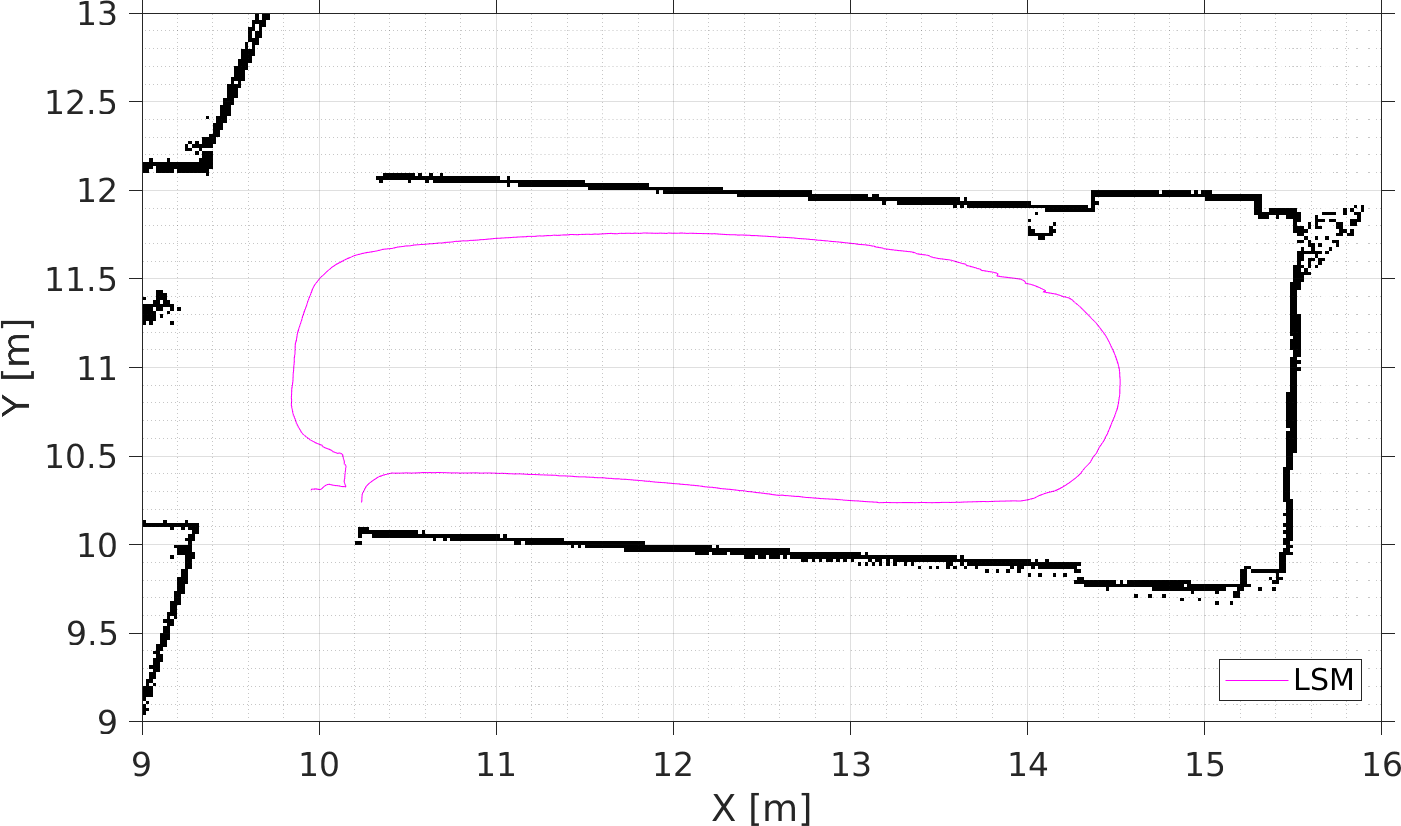
\includegraphics[width=\linewidth]{Record_2018-02-08-12-30-43_trajectory3}
		\caption{LSM}
		\label{fig:Record_2018-02-08-12-30-43_trajectory3}
	\end{subfigure}
	\hfill
	\begin{subfigure}{0.49\linewidth}
		\centering
		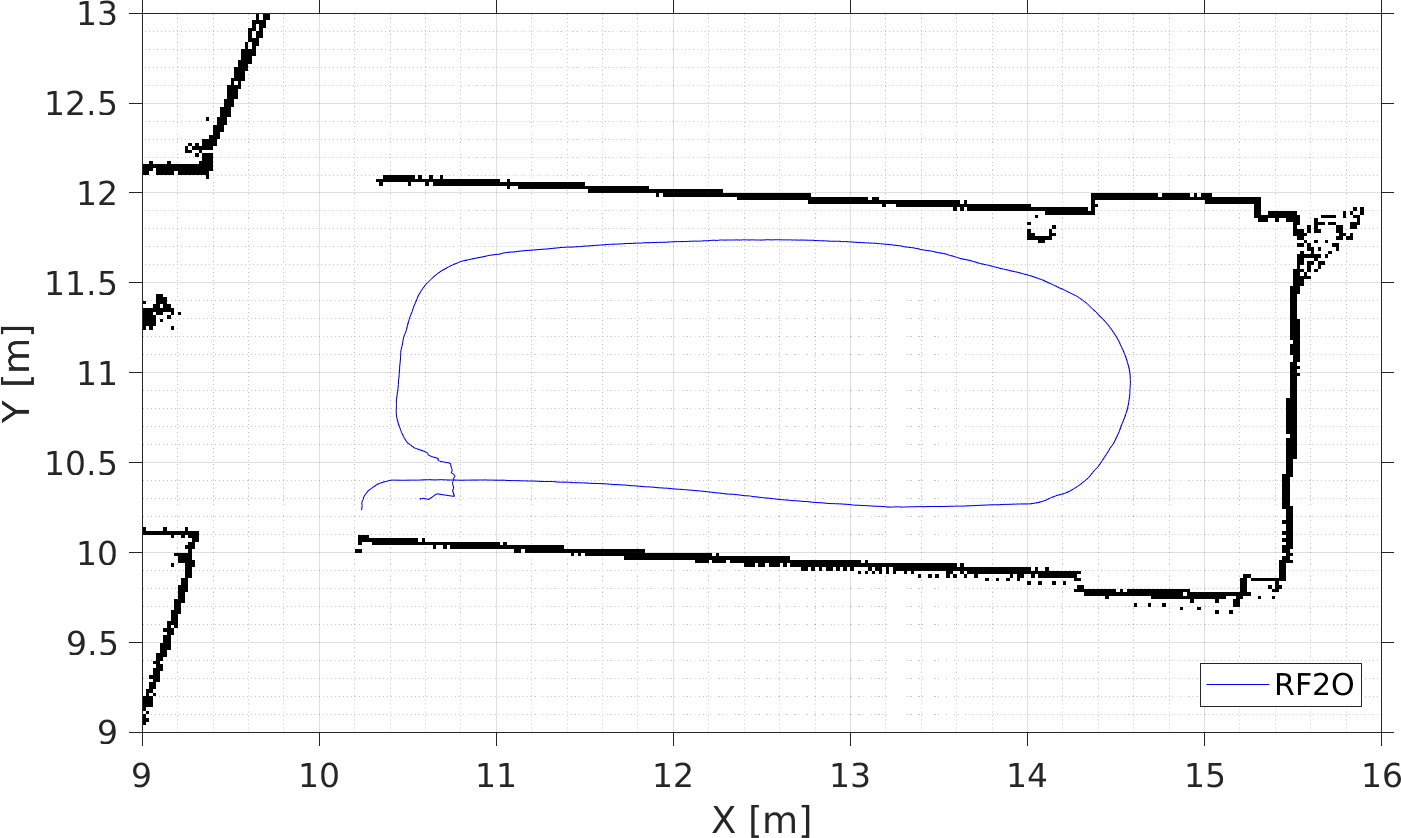
\includegraphics[width=\linewidth]{Record_2018-02-08-12-30-43_trajectory4}
		\caption{RF2O}
		\label{fig:Record_2018-02-08-12-30-43_trajectory4}
	\end{subfigure}
	\caption{Rechteckige Trajektorien der verschiedenen Odometriequellen.}
	\label{fig:Record_2018-02-08-12-30-43_trajectory}
\end{figure}


%%%%%%%%%%%%%%%%%%%%%%%%%%%%%%%%%%%%%%%%%%%%%%%%%%%%%%%%%%%%%%%%%%%%%%%%%%%%%%%%
%
%
%
%%%%%%%%%%
\chapter{Tabellen}

%\begin{sidewaystable}
\begin{table}[h]
	\centering
	\begin{tabular}{||c|c|l|c|l|c|r||} 
\hline
\gls{tag} & \gls{anchor} & Anbieter & Artikelnummer & Komponente & Anz. & Stckpr. \\\hline
\hline
\CheckedBox & \CheckedBox & Digi-Key & 1479-1002-1-ND & Decawave Limited & 1 & \SI{21.23}{\euro}\\
 & & & & DWM1000 & & \\\hline
\CheckedBox & \CheckedBox & Digi-Key & 1528-1040-ND & Adafruit Pro Trinket \SI{3}{\volt} & 1 & \SI{8.25}{\euro}\\\hline
\hline
\CheckedBox & \CheckedBox & Conrad & 1417697-62 & Kohleschicht-Widerstand & 1 & \SI{0.06}{\euro}\\
 & & & & \SI{10}{\kilo\ohm} & & \\\hline
\CheckedBox & \CheckedBox & Conrad & 1417644-62 & Kohleschicht-Widerstand & 4 & \SI{0.06}{\euro}\\
 & & & & \SI{180}{\ohm} & & \\\hline
\CheckedBox & \CheckedBox & Conrad & 180134-62 & LED Grün & 2 & \SI{0.25}{\euro}\\\hline
\CheckedBox & \CheckedBox & Conrad & 184756-62 & LED Rot & 2 & \SI{0.34}{\euro}\\\hline
\Square & \CheckedBox & Conrad & 251007-62 & Emmerich LiIon Akku & 1 & \SI{9.99}{\euro}\\
 & & & & ICR-18650 NH-SP & & \\\hline
\hline
\Square & \CheckedBox & EXP-Tech & EXP-R15-577 & Adafruit Pro Trinket & 1 & \SI{5.55}{\euro}\\
 & & & & LiPoly/LiIon Backpack & & \\\hline
\CheckedBox & \Square & EXP-Tech & EXP-R15-1157 & Adafruit CP2104 Friend & 1 & \SI{6.45}{\euro}\\\hline
\Square & \CheckedBox & EXP-Tech & EXP-R15-419 & Breadboard-friendly & 1 & \SI{1.20}{\euro}\\
 & & & & SPDT Slide Switch & & \\\hline
\Square & \CheckedBox & EXP-Tech & EXP-R15-1074 & JST 2-Pin Cable & 1 & \SI{0.80}{\euro}\\\hline

\hline
\CheckedBox & \CheckedBox & AISLER & -- & \acrlong{pcb} & 1 & \SI{7.74}{\euro}\\\hline
\hline
\multicolumn{6}{||r|}{Gesamtpreis für einen \gls{tag}:} & \SI{45.15}{\euro}\\\hline
\multicolumn{6}{||r|}{Gesamtpreis für einen \gls{anchor}:} & \SI{56.24}{\euro}\\\hline
	\end{tabular}
	\caption{Materialkosten pro \glsentrytext{tag} bzw. \glsentrytext{anchor}.}
	\label{tab:kosten_pro_modul}
%\end{sidewaystable}
\end{table}


% ------------------------------------------------------------------------------
% Evaluation - Entfernungsmessung
% ------------------------------------------------------------------------------

\begin{table}
	\centering
	\begin{tabular}{||c||ccc||cc||c||}
\hline
Entfernung & $\overline{x}$ & $\sigma$ & $SE_{\overline{x}}$ & Min & Max & Bias \\
{[}\si{\meter}{]} & {[}\si{\meter}{]} & {[}\si{\meter}{]} & {[}\si{\meter}{]} & {[}\si{\meter}{]} & {[}\si{\meter}{]} & {[}\si{\meter}{]} \\
\hline
\hline
\num{1.0} & \num{1.222} & \num{0.018} & \num{0.0008} & \num{1.130} & \num{1.270} & \num{0.222} \\
\num{1.5} & \num{1.760} & \num{0.017} & \num{0.0007} & \num{1.680} & \num{1.820} & \num{0.260} \\
\num{2.0} & \num{2.262} & \num{0.019} & \num{0.0008} & \num{2.220} & \num{2.350} & \num{0.262} \\
\num{2.5} & \num{2.729} & \num{0.018} & \num{0.0008} & \num{2.670} & \num{2.790} & \num{0.229} \\
\num{3.0} & \num{3.240} & \num{0.021} & \num{0.0009} & \num{3.190} & \num{3.300} & \num{0.240} \\
\num{3.5} & \num{3.758} & \num{0.021} & \num{0.0009} & \num{3.710} & \num{3.810} & \num{0.258} \\
\num{4.0} & \num{4.210} & \num{0.019} & \num{0.0008} & \num{4.150} & \num{4.260} & \num{0.210} \\
\num{4.5} & \num{4.702} & \num{0.018} & \num{0.0008} & \num{4.640} & \num{4.760} & \num{0.202} \\
\num{5.0} & \num{5.182} & \num{0.019} & \num{0.0008} & \num{5.120} & \num{5.260} & \num{0.182} \\
\num{5.5} & \num{5.690} & \num{0.020} & \num{0.0009} & \num{5.630} & \num{5.750} & \num{0.190} \\
\num{6.0} & \num{6.205} & \num{0.021} & \num{0.0009} & \num{6.120} & \num{6.270} & \num{0.205} \\
\num{6.5} & \num{6.714} & \num{0.022} & \num{0.0010} & \num{6.660} & \num{6.810} & \num{0.214} \\
\num{7.0} & \num{7.227} & \num{0.025} & \num{0.0011} & \num{7.160} & \num{7.310} & \num{0.227} \\
\num{7.5} & \num{7.735} & \num{0.026} & \num{0.0011} & \num{7.670} & \num{7.810} & \num{0.235} \\
\num{8.0} & \num{8.209} & \num{0.023} & \num{0.0010} & \num{8.140} & \num{8.280} & \num{0.209} \\
\num{8.5} & \num{8.707} & \num{0.023} & \num{0.0010} & \num{8.630} & \num{8.770} & \num{0.207} \\
\num{9.0} & \num{9.204} & \num{0.023} & \num{0.0010} & \num{9.120} & \num{9.290} & \num{0.204} \\
\hline
	\end{tabular}
	\caption{Stochastische Merkmale der \glsentryshort{los}--Entfernungsmessung.}
	\label{tab:entfernungsmessung_2018_01_20_los}
\end{table}

\begin{table}
	\centering
	\begin{tabular}{||c||ccc||cc||c||}
\hline
Entfernung & $\overline{x}$ & $\sigma$ & $SE_{\overline{x}}$ & Min & Max & Bias \\
{[}\si{\meter}{]} & {[}\si{\meter}{]} & {[}\si{\meter}{]} & {[}\si{\meter}{]} & {[}\si{\meter}{]} & {[}\si{\meter}{]} & {[}\si{\meter}{]} \\
\hline
\hline
\num{1.0} & \num{1.617} & \num{0.164} & \num{0.0073} & \num{1.170} & \num{2.160} & \num{0.617} \\
\num{1.5} & \num{2.026} & \num{0.193} & \num{0.0086} & \num{1.520} & \num{2.340} & \num{0.526} \\
\num{2.0} & \num{2.471} & \num{0.192} & \num{0.0086} & \num{2.120} & \num{2.900} & \num{0.471} \\
\num{2.5} & \num{2.681} & \num{0.042} & \num{0.0019} & \num{2.590} & \num{3.030} & \num{0.181} \\
\num{3.0} & \num{3.139} & \num{0.039} & \num{0.0017} & \num{3.060} & \num{3.500} & \num{0.139} \\
\num{3.5} & \num{3.796} & \num{0.154} & \num{0.0069} & \num{3.580} & \num{4.420} & \num{0.296} \\
\num{4.0} & \num{4.384} & \num{0.215} & \num{0.0096} & \num{4.060} & \num{5.000} & \num{0.384} \\
\num{4.5} & \num{4.928} & \num{0.212} & \num{0.0095} & \num{4.550} & \num{5.940} & \num{0.428} \\
\num{5.0} & \num{5.786} & \num{0.111} & \num{0.0050} & \num{5.310} & \num{5.940} & \num{0.786} \\
\num{5.5} & \num{6.530} & \num{0.263} & \num{0.0118} & \num{5.800} & \num{7.140} & \num{1.030} \\
\num{6.0} & \num{6.879} & \num{0.054} & \num{0.0024} & \num{6.740} & \num{7.300} & \num{0.879} \\
\num{6.5} & \num{7.364} & \num{0.060} & \num{0.0027} & \num{7.240} & \num{7.850} & \num{0.864} \\
\num{7.0} & \num{7.819} & \num{0.076} & \num{0.0034} & \num{7.690} & \num{8.690} & \num{0.819} \\
\num{7.5} & \num{8.466} & \num{0.193} & \num{0.0086} & \num{8.210} & \num{9.750} & \num{0.966} \\
\num{8.0} & \num{8.907} & \num{0.125} & \num{0.0056} & \num{8.750} & \num{9.540} & \num{0.907} \\
\num{8.5} & \num{9.626} & \num{0.340} & \num{0.0152} & \num{9.190} & \num{11.010} & \num{1.126} \\
\num{9.0} & \num{10.680} & \num{0.315} & \num{0.0141} & \num{9.980} & \num{11.680} & \num{1.680} \\
\hline
	\end{tabular}
	\caption{Stochastische Merkmale der \glsentryshort{nlos}--Entfernungsmessung mit einem wassergefüllten Kunststoffbehälter.}
	\label{tab:entfernungsmessung_2018_01_20_nlos_water}
\end{table}

\begin{table}
	\centering
	\begin{tabular}{||c||ccc||cc||c||}
\hline
Entfernung & $\overline{x}$ & $\sigma$ & $SE_{\overline{x}}$ & Min & Max & Bias \\
{[}\si{\meter}{]} & {[}\si{\meter}{]} & {[}\si{\meter}{]} & {[}\si{\meter}{]} & {[}\si{\meter}{]} & {[}\si{\meter}{]} & {[}\si{\meter}{]} \\
\hline
\hline
\num{1.0} & \num{1.285} & \num{0.021} & \num{0.0009} & \num{1.230} & \num{1.360} & \num{0.285} \\
\num{1.5} & \num{1.770} & \num{0.019} & \num{0.0008} & \num{1.710} & \num{1.840} & \num{0.270} \\
\num{2.0} & \num{2.305} & \num{0.020} & \num{0.0009} & \num{2.240} & \num{2.360} & \num{0.305} \\
\num{2.5} & \num{2.803} & \num{0.020} & \num{0.0009} & \num{2.740} & \num{2.870} & \num{0.303} \\
\num{3.0} & \num{3.303} & \num{0.022} & \num{0.0010} & \num{3.250} & \num{3.370} & \num{0.303} \\
\num{3.5} & \num{3.816} & \num{0.022} & \num{0.0010} & \num{3.750} & \num{3.880} & \num{0.316} \\
\num{4.0} & \num{4.269} & \num{0.024} & \num{0.0011} & \num{4.170} & \num{4.340} & \num{0.269} \\
\num{4.5} & \num{4.728} & \num{0.021} & \num{0.0010} & \num{4.670} & \num{4.860} & \num{0.228} \\
\num{5.0} & \num{5.250} & \num{0.023} & \num{0.0010} & \num{5.180} & \num{5.320} & \num{0.250} \\
\num{5.5} & \num{5.707} & \num{0.023} & \num{0.0010} & \num{5.630} & \num{5.780} & \num{0.207} \\
\num{6.0} & \num{6.276} & \num{0.032} & \num{0.0014} & \num{6.150} & \num{6.360} & \num{0.276} \\
\num{6.5} & \num{6.801} & \num{0.029} & \num{0.0013} & \num{6.730} & \num{6.890} & \num{0.301} \\
\num{7.0} & \num{7.253} & \num{0.040} & \num{0.0018} & \num{7.150} & \num{7.560} & \num{0.253} \\
\num{7.5} & \num{7.788} & \num{0.055} & \num{0.0025} & \num{7.650} & \num{8.140} & \num{0.288} \\
\num{8.0} & \num{8.290} & \num{0.030} & \num{0.0013} & \num{8.200} & \num{8.400} & \num{0.290} \\
\num{8.5} & \num{9.066} & \num{0.379} & \num{0.0169} & \num{8.630} & \num{10.280} & \num{0.566} \\
\num{9.0} & \num{9.490} & \num{0.237} & \num{0.0106} & \num{9.110} & \num{10.250} & \num{0.490} \\
\hline
	\end{tabular}
	\caption{Stochastische Merkmale der \glsentryshort{nlos}--Entfernungsmessung mit einem Aluminiumblech in einer Entfernung von \SI{50}{\centi\meter}.}
	\label{tab:entfernungsmessung_2018_01_20_nlos_metal}
\end{table}

\begin{table}
	\centering
	\begin{tabular}{||c||ccc||cc||c||}
\hline
Entfernung & $\overline{x}$ & $\sigma$ & $SE_{\overline{x}}$ & Min & Max & Bias \\
{[}\si{\meter}{]} & {[}\si{\meter}{]} & {[}\si{\meter}{]} & {[}\si{\meter}{]} & {[}\si{\meter}{]} & {[}\si{\meter}{]} & {[}\si{\meter}{]} \\
\hline
\hline
\num{1.0} & \num{1.722} & \num{0.234} & \num{0.0105} & \num{1.320} & \num{2.350} & \num{0.722} \\
\num{1.5} & \num{1.744} & \num{0.056} & \num{0.0025} & \num{1.660} & \num{2.410} & \num{0.244} \\
\num{2.0} & \num{2.260} & \num{0.028} & \num{0.0012} & \num{2.190} & \num{2.360} & \num{0.260} \\
\num{2.5} & \num{2.800} & \num{0.025} & \num{0.0011} & \num{2.730} & \num{2.870} & \num{0.300} \\
\num{3.0} & \num{3.284} & \num{0.025} & \num{0.0011} & \num{3.210} & \num{3.390} & \num{0.284} \\
\num{3.5} & \num{3.803} & \num{0.034} & \num{0.0015} & \num{3.730} & \num{4.290} & \num{0.303} \\
\num{4.0} & \num{4.285} & \num{0.029} & \num{0.0013} & \num{4.210} & \num{4.380} & \num{0.285} \\
\num{4.5} & \num{4.754} & \num{0.033} & \num{0.0015} & \num{4.660} & \num{5.030} & \num{0.254} \\
\num{5.0} & \num{5.320} & \num{0.166} & \num{0.0074} & \num{5.140} & \num{6.370} & \num{0.320} \\
\num{5.5} & \num{6.113} & \num{0.381} & \num{0.0170} & \num{5.690} & \num{7.790} & \num{0.613} \\
\num{6.0} & \num{6.538} & \num{0.339} & \num{0.0152} & \num{6.160} & \num{7.700} & \num{0.538} \\
\num{6.5} & \num{7.311} & \num{0.382} & \num{0.0171} & \num{6.650} & \num{8.760} & \num{0.811} \\
\num{7.0} & \num{8.531} & \num{0.342} & \num{0.0153} & \num{7.500} & \num{9.190} & \num{1.531} \\
\num{7.5} & \num{8.783} & \num{0.285} & \num{0.0128} & \num{8.020} & \num{9.750} & \num{1.283} \\
\num{8.0} & \num{9.543} & \num{0.077} & \num{0.0034} & \num{9.190} & \num{10.300} & \num{1.543} \\
\num{8.5} & \num{10.089} & \num{0.230} & \num{0.0103} & \num{9.480} & \num{10.740} & \num{1.589} \\
\num{9.0} & \num{10.622} & \num{0.353} & \num{0.0158} & \num{10.160} & \num{11.500} & \num{1.622} \\
\hline
	\end{tabular}
	\caption{Stochastische Merkmale der \Gls{nlos}--Entfernungsmessung mit einem Aluminiumblech in einer Entfernung von \SI{5}{\centi\meter}.}
	\label{tab:entfernungsmessung_2018_01_20_nlos_metal2}
\end{table}


%%%%%%%%%%%%%%%%%%%%%%%%%%%%%%%%%%%%%%%%%%%%%%%%%%%%%%%%%%%%%%%%%%%%%%%%%%%%%%%%
%
%
%
%%%%%%%%%%
%\chapter{Auflistungen}
%
%
%\begin{listing}
%	\begin{minted}[frame=single]{xml}
%<node pkg="joy" type="joy_node" name="joy_node">
%
%  <param name="dev" type="string" value="/dev/input/js0" />
%</node>
%	\end{minted}
%	\unskip
%	\caption{Konfiguration des \textit{joy\_node}.}
%	\label{lst:joy_node}
%\end{listing}
%
%
%\begin{listing}
%	\begin{minted}[frame=single]{xml}
%<node pkg="hector_trajectory_server" type="hector_trajectory_server" name="hector_trajectory_server_node">
%
%  <param name="target_frame_name" value="map"/>
%  <param name="source_frame_name" value="base_link" />
%  <param name="trajectory_update_rate" value="10.0" />
%  <param name="trajectory_publish_rate" value="10"/>
%</node>
%	\end{minted}
%	\unskip
%	\caption{Konfiguration der \textit{hector\_trajectory\_server}.}
%	\label{lst:hector_trajectory_server_node}
%\end{listing}


\end{appendices}